\documentclass[conference]{IEEEtran}
\IEEEoverridecommandlockouts
% The preceding line is only needed to identify funding in the first footnote. If that is unneeded, please comment it out.
\usepackage{cite}
\usepackage{amsmath,amssymb,amsfonts}
\usepackage{algorithmic}
\usepackage{graphicx}
\usepackage{textcomp}
\usepackage{xcolor}
\def\BibTeX{{\rm B\kern-.05em{\sc i\kern-.025em b}\kern-.08em
    T\kern-.1667em\lower.7ex\hbox{E}\kern-.125emX}}
\begin{document}

\title{Handwritten Digit Recognition using Artificial Neural Networks }



\author{\IEEEauthorblockN{Kumari Pooja}
\IEEEauthorblockA{\textit{3rd year - Avionics} \\
\textit{IIST}\\
poojakumari.iist@gmail.com}
\and
\IEEEauthorblockN{Pragya Shah}
\IEEEauthorblockA{\textit{3rd year - Avionics} \\
\textit{IIST}\\
pragyashree19@gmail.com}

}

\maketitle

\begin{abstract}
Handwritten digits recongnition has not been easy for computers while we humans are really good at it. This report gives an idea to enable computers to recognize digits to a fairly high accuracy using Artificial Neural Networks. The MNIST data are used for training and testing the performance of the trained net. The input of the network consists of segmented grey digits image. We also explore the effect of architecture and hyperparameters on the classifier's performance in terms of computation cost, training time and accuracy. Our experiments shows which architecture of the networks will give the promising accuracy.
   
\end{abstract}

\begin{IEEEkeywords}

Artificial Neural Network (ANN), MNIST, Back Propagation (BP), Gradient Descent, Mini-batch Learning
\end{IEEEkeywords}

\section{Introduction}
Handwritten digit recognition is majorly used in OCR applications. It helps to do postal mail sorting, bank check processing, form data entry, etc. The accuracy and speed is the pivotal for the overall performance in these type of applications. The objective of this reposrt is to show that backpropagation (BP) networks can be applied to real image-recognition problems without a large, complex preprocessing stage requiring detailed engineering. Unlike other image proseccing techniques, the learning network is directly fed with image's pixels, rather than feature vectors, thus demonstrating the ability of BP networks to deal with large amounts of low level information. Previous work done on simple digit images show that the architecture of the network strongly influences the network's generalization ability.The basic design principle is to minimize the number 
of free parameters that must be determined by the learning algorithm, without overly reducing the computational power of the network. 


\section{Related works}
Similar work has been done in the past focusing on various types of classifiers and their corresponding error rate. A MLP
with a single hidden layer of 800 units achieved 0.70\% error [3]. However, more complex methods listed on the MNIST web page always seemed to outperform MLPs, and the general trend went towards more and more complex variants of Support Vector Machines or SVMs [4] and combinations of NNs and SVMs [5] etc. Convolutional neural networks (CNNs) achieved a record-breaking 0.40\% error rate [3], using novel elastic training image deformations. Another modle which are used for classification are LeNet 1 [2] with 1.7\% error, LeNet4 with 1.1\% error, Large fully connected multi-layer neural network with 1.6\% error on MNIST test set.  
\section{Methodology}
\subsection{Architecture}
The simple, fully connected, multilayer feedforward architecture of Artificial neural network has been used. The input layer consists of the number of pixels contained in the image being processed. The input layer is built only to fanout each input data to all the nodes of the first hidden layer.
\begin{figure}[h]
	\centering
	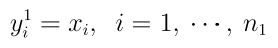
\includegraphics[width=0.45\linewidth]{inlayer}
\end{figure}

Output layer consists of 10 nodes, one for each digit. The node with the highest output denotes the digit into which the input image has been classified. In between lie the hidden layer. Each node uses the sigmoid activation function.
\begin{figure}[h]
	\centering
	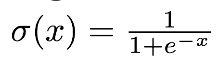
\includegraphics[width=0.3\linewidth]{sigmoid}
\end{figure}

\subsection{Loss function}
The loss function being used is the square of the error betwen the output of the network and the desired (or labled) output of the training example.
\begin{figure}[h]
	\centering
	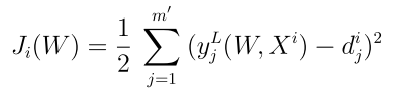
\includegraphics[width=0.65\linewidth]{loss}
\end{figure}

\subsection{Weight Initialization}
The architecture of the networks used did not require to be deep as we are dealing with only ten classes of low resolution digits. Thus weight initialization was done by small random number generated from a normal distribution. It is however obvious that for handling more complex data like faces that have several details, deep nets are required. Then we need to consider better ways to initialize the weights and also employ techniques like weight dropping and batch normalization. Same is the case when we have too many classes of data.

\subsection{Gradient Descent and Back Propagation}
For updating the weights - Gradient descent method is being used. Though it gives a local minima for any function, it is fairly useful most of the time. 
\begin{figure}[h]
	\centering
	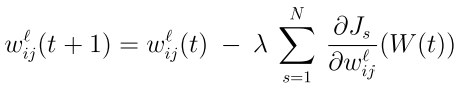
\includegraphics[width=0.75\linewidth]{update}
\end{figure}

This introduces a new hyperparameter called the learning rate of the network. It must be choosen carefully as too small a value will slow down convergence to a painfully slow rate while a very large value might not allow the model to converge due to overshoots.

For the gradient descent, loss and y (output) both need to be differentiable, i.e., our activation function must be differentiable, thus we are using sigmoid activations at each node.

The gradient is calculated by a method known as backpropagation where the error due to each node is back propagated through the network to compute the error at the lower levels of the network. This is the most powerfull tool of our system that enables the weights to automatically adjust themselves by observing the deviation of the network's outupt from the lables of the training data and the effect each weight has over this deviation.

\begin{figure}[h]
	\centering
	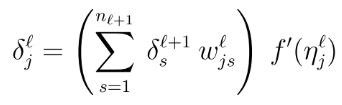
\includegraphics[width=0.55\linewidth]{delta}
\end{figure}
\begin{figure}[h]
	\centering
	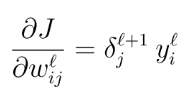
\includegraphics[width=0.3\linewidth]{grad}
\end{figure}

\subsection{Minibatch Learning}
To facilitate fast and steady convergence of the network to the local minima of the loss function, we have introduces minibatch learning algorithm for gradient descent. In this method, the weights and bias of the network are updated much more frequently than in the batch learning case. The batch is shuffled and divided into x number of smaller batches of equal size. After scanning through all the data points in a minibatch, the weights are updated. Thus within one epoch, the weights and bias are updated x times as compared to the batch learning case where they would be updated only once in an epoch. This enables the weights to stablize themselves in fewer number of epochs and also cuts down the time required for training immensely.
\section{Dataset}
In order to obtain a database more typical of real-world applications, we have used US Modified National Institute of Standards and Technology (MNIST).[2] The MNIST data comes in two parts. The first part contains 60,000 images to be used as training data. These images are scanned handwriting samples from 250 people, half of whom were US Census Bureau employees, and half of whom were high school students. The images are greyscale and 28 by 28 pixels in size. The second part of the MNIST data set is 10,000 images to be used as test data. Again, these are 28 by 28 greyscale images. We'll use the test data to evaluate how well our neural network has learned to recognize digits. To make this a good test of performance, the test data was taken from a different set of 250 people than the original training data (albeit still a group split between Census Bureau employees and high school students). This helps give us confidence that our system can recognize digits from people whose writing it didn't see during training. The sample of a image is shown in fig. 1.\newline

The general format of our model is as follows. We take (28x28) segmented grey image of a digit change it into vector format of 784x1 and give as an input to the ANN. Using these training images and their lables the network learns its bias and weights to each node. 
\begin{figure}[h]
	\centering
	\includegraphics[width=\linewidth]{"MNIST sample image"}
	\caption{MNIST sample Image}
	\label{Fig:1}
\end{figure}
\section{Experiments and Results}
\subsection{Determining Hyperparameters:}
Hyperparameters are free parameters which are not learned by the network via BP and Gradient Descent, they are determined by the developer of the network as per his requirements. Some of these are - number of hidden layers in the network, number of nodes in the different hidden layers, learning rate of network, minibatch size of the training data, number of epocs in training of the network etc. As of now, there are no hard and fast rules to provide one with the best set of hyperparameters for ones network. They are mostly determined by hit and trial method. We conducted tests by varying each of the above mentioned parameters one by one and observed the performance of the network interms of accuracy and training time. Here are the results for the experiment (you may need to zoom in to see the numbers)
\begin{figure}[h]
	\centering
	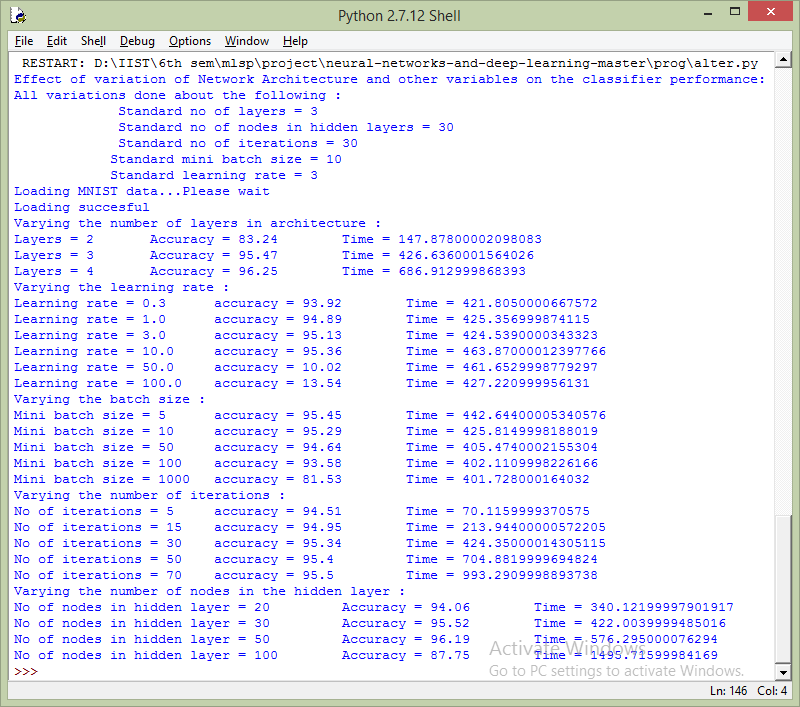
\includegraphics[width=\linewidth]{vary}
	\caption{Output of alter.py - Network Performance on Varying Hyperparameters}
\end{figure}
\begin{figure}[h]
	\centering
	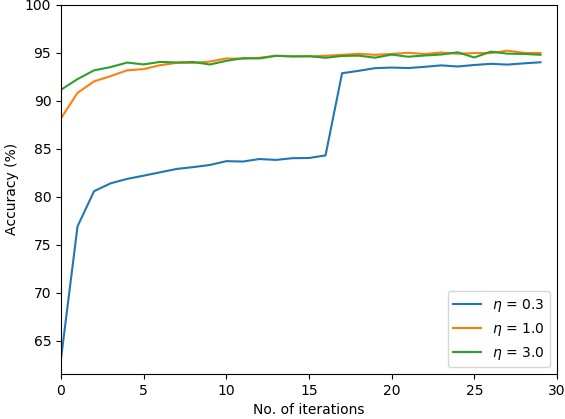
\includegraphics[width=\linewidth]{multi_eta_accuracy}
	\caption{Accuracy trend with increasing no of epocs for various learning rates}
\end{figure}
\begin{figure}[h]
	\centering
	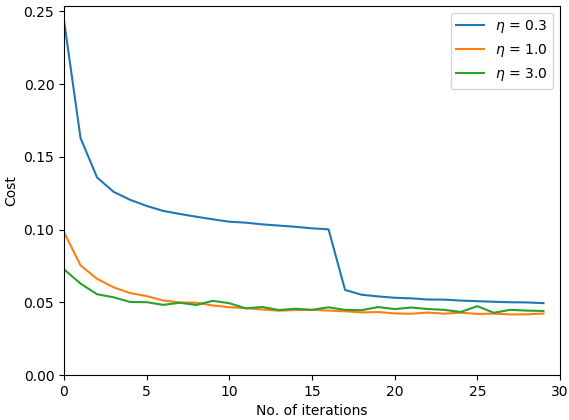
\includegraphics[width=\linewidth]{multi_eta_cost}
	\caption{Cost or Loss(J) trend with increasing epocs for various learning rates}
\end{figure}

Observing the outputs, numerous inferences were drawn.
\begin{enumerate}
\item Increasing number of hidden layers in the network enhances the accuracy but the time needed for training grows multifold. Even the accuracy saturates after a certain number of hidden layers and further increase in layers may cause a decrease instead.
\item By varying the learning rate, we can find a goldilocks zone and fine tune it's value to get best results. Outside this zone, the accuracy falls off rapidly with little effect on training time
\item From the accuracy and loss graphs, we can see that graphs of learning rates of the optimal zone stablize within a very small number of epocs while performance of those outside this zone varies heavily, depending upon the number of epocs and other factors.
\item Increasing minibatch size leads to decrease in accuracy as the number of times weights are being updated decreases. Same reason is responsible for the slight decrease in training time. Now to maintain the accuracy, number of epocs must be increased.
\item With other factors constant, increase in number of epocs shows no improvement in accuracy and an obvious increase in training time is noted. This indicates that in this case, the other hyperparameters are such that the network has converged well before all the epocs got over If epocs are taken down to very low numbers when the network is still trying to stablize itself, a considerable change in accuracy will be seen.
\item Like the learning rate, the number of nodes in a layer also has a goldilocks zone within which we can fine tune it as per requirements. A steady rise in training time is seen with increasing number of nodes.
\end{enumerate}

Thus, a developer can take clues from such experiments as per what will suit his objective best. Mostly training time is not a concern as once the model is trained, it will not matter. But while the system is in development and debugging phase, we would like the training time to be managable, or we may run our network on a smaller training data for the debudding period.
\subsection{Trends of an architecture:}
Next we observed the trends of an architecture with following specifications:

Number of hidden layer - 1

Number of hidden layer nodes - 30

No of epocs - 30

Mini batch size - 10

Learning rate - 3.0

These parameters were chosen after observing the outcome of the previous experiments. They were most suitable for us, giving us a high accuracy of about 95.03\% and a moderate training time to enable us to make changes to our network. 


\begin{figure}[h]
	\centering
	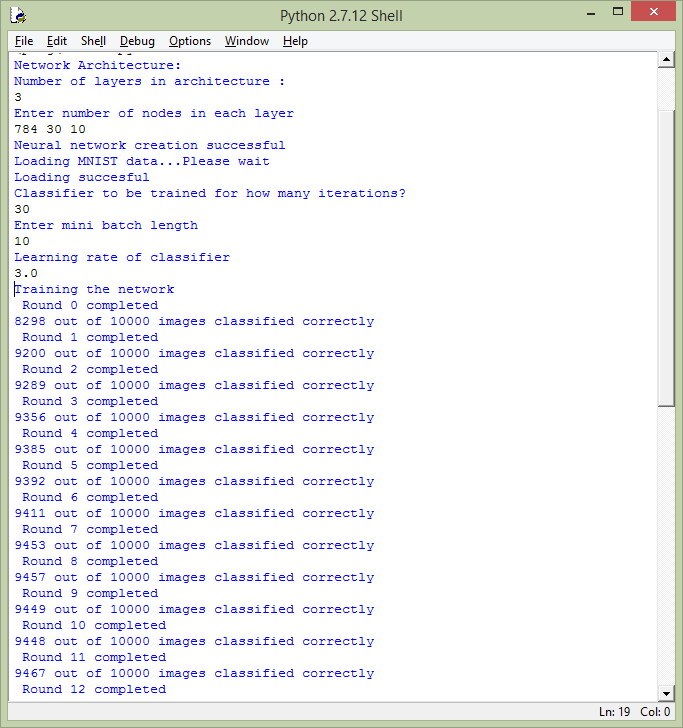
\includegraphics[width=\linewidth]{custom}
	\caption{O/P of custom.py-Network Performance for given Hyperparameters(1)}
\end{figure}
\begin{figure}[h]
	\centering
	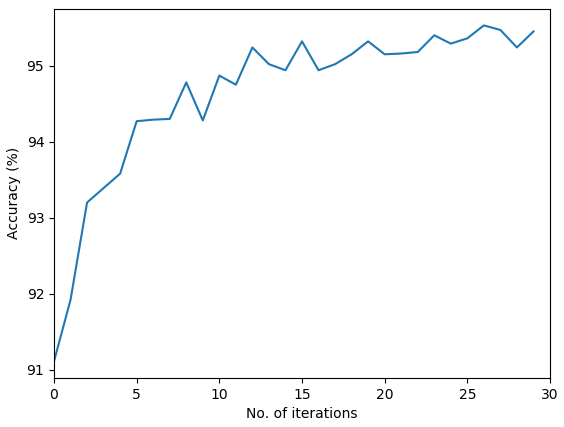
\includegraphics[width=\linewidth]{Custom_Accuracy}
	\caption{Accuracy trend with increasing no of epocs}
\end{figure}
\begin{figure}[h]
	\centering
	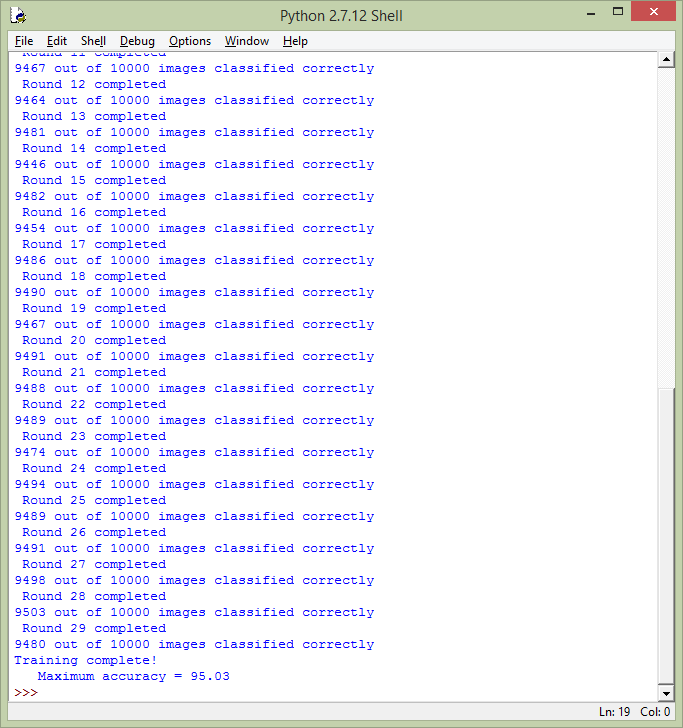
\includegraphics[width=\linewidth]{custom2}
	\caption{O/P of custom.py-Network Performance for given Hyperparameters(2)}
\end{figure}
\begin{figure}[h]
	\centering
	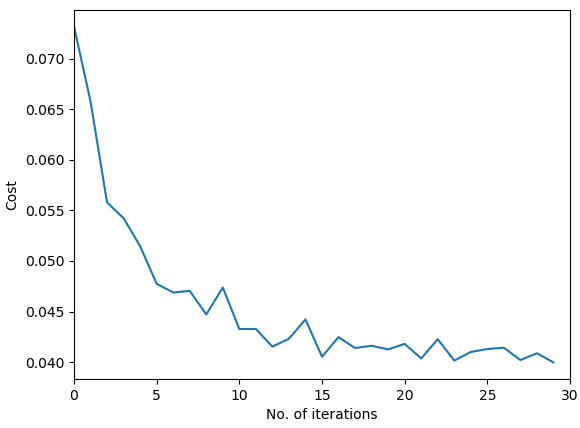
\includegraphics[width=\linewidth]{Custom_cost}
	\caption{Cost or Loss(J) trend with increasing epocs}
\end{figure}

It can be seen that accuracy and loss appear complementary to each other. The accuracy increases exponentialy with epocs and starts to saturate at later iterations. Similarly loss function falls off exponentilly with epocs and reaches a minima below which it cannot deacrease.

For this network,

Number of weights = 784*30 + 30*10 = 23,820

Number of bias = 30 + 10 = 40

Thus, Total Number of parameters = 23,820 + 40 = 23,860

Also, we have a training set of 60,000 images, mini batch size of 10 and 30 epocs. Thus weight and bias matrix are updated (30*60000/10 = ) 1,80,000 times during training!!

Maximum Accuracy of this classifier = 95.03\%

\section{Conclusions}
Through this project, we examined and proved the ability of Multilayer feedforward neural networks. They are efficient for handling low level data like raw pixels without any preprocessing like feature extraction or spatial information. An ordinary three layer network provided us with an amazing accuracy of 95.03\%. Though it may be difficult to decide which hyperprameters would work best for the network at first, tinkering around with them and observing the effect of change in one of them over the performance of the system can be helpful. Using techniques like minibacth learning and gradient descent will make training much more faster and easier.

\subsection{Future Scope}
Much more work can still be done in this project. As sugested by our Professor Dr. Deepak Mishra, we are trying to observe how the model responds to rotated images from the same dataset and how we can remove the orientation dependance of the classifier. We will be repeating the experiments with different activation functions like relu, etc and analyse the advantages and shortcomings. Better weight initialization techniques can also be explored and batch normalization and weight dropping methods can be used to classify images of more complex objects as well.

The scope of ANN are unlimited and they are a very basic immitation of the human brain. Many of the simpler problems can be solved by this algorithm far more easily than it can be done by its mathematically complex competitors like SVM etc. But one must remmember, in case of similar performance, one must choose the model that is simpler in implementation, and ANNs are powerful yet the simplest of all Machine Learning algorithms.
\section*{Acknowledgment}
We would like to express our deep gratitude and sincere thanks to Dr. Deepak Mishra, for giving us the opportunity to do an interesting project. We are grateful for the constant support and encouragement he provided. Youre timely help, advice on all matters and friendly behavior is truely appreciated Sir. We would also like to extend our greatfullness to our batchmates for their cooperation and involvement in the presentation. \newline
We also express our gratitude towards IIST, Thiruvananthapuram for providing us a congenial environment to work with.\newline
Above all, We thank God Almighty who enabled us with philosophy, perception and motivation to present this work.\newline

\begin{thebibliography}{00}
\bibitem{b1} LeCun Y., Bottou, L., Bengio, Y. \& Haffner, P. (1998). Gradient-Based Learning Applied to Document Recognition. Proceedings of the IEEE, 86, 309-318.
\bibitem{b2} L. Bottou, C. Cortes, H. Drucker, I. Guyon, LeCun Y. (2002). Comparison of classifier methods: a case study in handwritten digit recognition. Proceedings of the IEEE.
\bibitem{b3} Simard, P.Y., Steinkraus, D. \& Platt, J.C. (2003). Best Practices for Convolutional Neural Networks Applied to Visual Document Analysis. Intl. Conf. Document Analysis and Recognition, 958 – 962.
\bibitem{b4} Decoste, D. \& Scholkopf, B. (2002). Training Invariant Support Vector Machines. Machine learning, 46, 161 – 190.
\bibitem{b5} Lauer, F., Suen, C. \& Bloch, G. (2007). A trainable feature extractor for handwritten digit recognition. Pattern Recognition, 40, 1816 – 1824.
\bibitem{b6} NumPY
\end{thebibliography}
\vspace{12pt}


\end{document}
